% figures/autonomy-loop-map.tex — F2 v3 (layout-aligned revision)
% Unit of analysis and evidence classifications are unchanged; only visual layout/alignment is revised.
\begin{figure*}[t]
\centering
\resizebox{\textwidth}{!}{%
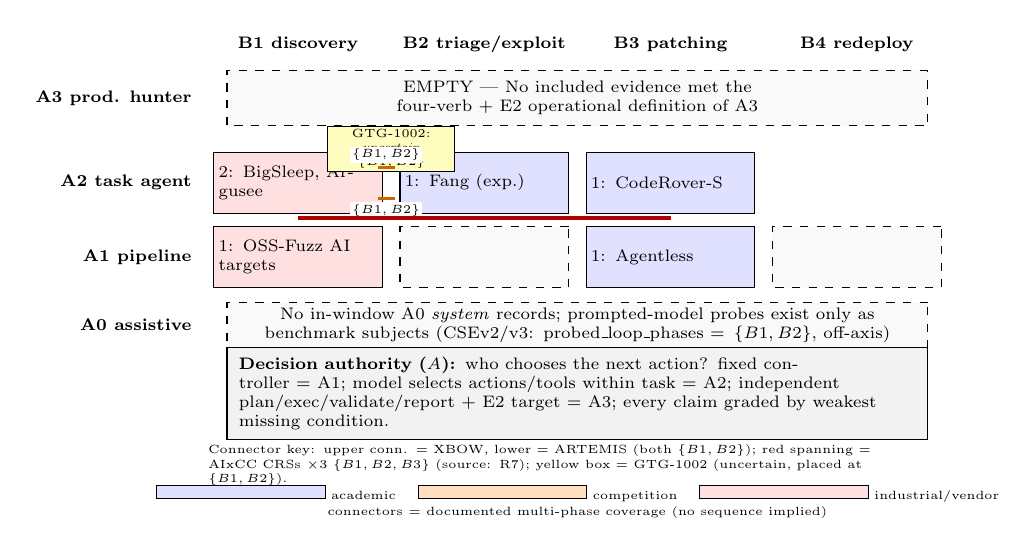
\begin{tikzpicture}[
  cell/.style={draw,align=left,font=\scriptsize,text width=2.35cm,minimum height=0.90cm,inner sep=2pt},
  acad/.style={cell,fill=blue!12}, comp/.style={cell,fill=orange!25},
  ind/.style={cell,fill=red!12}, empt/.style={cell,dashed,fill=gray!5},
  ctx/.style={draw,fill=gray!10,font=\scriptsize,align=left,text width=10.0cm,inner sep=4pt},
  lab/.style={font=\scriptsize\bfseries},
  conn/.style={-,very thick,orange!80!black},
  scale=0.86,transform shape]

% Phase headers: one shared grid.
\node[lab] at (0.0,4.30) {B1 discovery};
\node[lab] at (2.75,4.30) {B2 triage/exploit};
\node[lab] at (5.5,4.30) {B3 patching};
\node[lab] at (8.25,4.30) {B4 redeploy};

% Autonomy labels.
\node[lab,anchor=east] at (-1.45,3.50) {A3 prod. hunter};
\node[lab,anchor=east] at (-1.45,2.25) {A2 task agent};
\node[lab,anchor=east] at (-1.45,1.15) {A1 pipeline};
\node[lab,anchor=east] at (-1.45,0.15) {A0 assistive};

% A3 row.
\node[empt,minimum width=10.35cm,minimum height=0.82cm,text width=10.0cm,align=center] at (4.125,3.50)
 {\scriptsize EMPTY --- No included evidence met the four-verb $+$ E2 operational definition of A3};

% A2 row.
\node[ind]  at (0.0,2.25) {2: BigSleep, Argusee};
\node[acad] at (2.75,2.25) {1: Fang (exp.)};
\node[acad] at (5.5,2.25) {1: CodeRover-S};
% GTG-1002: narrow yellow label in B1--B2 gutter (its loop phases).
\node[font=\tiny,anchor=center,draw,fill=yellow!25,align=center,text width=1.8cm,minimum height=0.55cm,inner sep=1pt]
  at (1.375,2.75) {GTG-1002: \emph{uncertain} $\{B1,B2\}$};

% Neutral documented-coverage connectors.  The line itself stays entirely in the gutter;
% the phase-set labels sit in the whitespace immediately adjacent to that gutter.
\draw[conn] (1.175,2.48) -- (1.425,2.48);
\node[font=\tiny,anchor=south,fill=white,inner sep=1pt] at (1.30,2.53) {$\{B1,B2\}$};
\draw[conn] (1.175,2.02) -- (1.425,2.02);
\node[font=\tiny,anchor=north,fill=white,inner sep=1pt] at (1.30,1.97) {$\{B1,B2\}$};
% AIxCC is a documented B1--B3 multi-phase record; red connector spans B1--B3.
\draw[conn,red!70!black] (0.0,1.73) -- (5.5,1.73);


% A1 row.
\node[ind]  at (0.0,1.15) {1: OSS-Fuzz AI targets};
\node[empt] at (2.75,1.15) {};
\node[acad] at (5.5,1.15) {1: Agentless};
\node[empt] at (8.25,1.15) {};

% A0 note, kept inside the same B-grid.
\node[empt,minimum width=10.35cm,minimum height=0.62cm,text width=10.0cm,align=center] at (4.125,0.15)
 {\scriptsize No in-window A0 \emph{system} records; prompted-model probes exist only as benchmark
  subjects (CSEv2/v3: probed\_loop\_phases $=\{B1,B2\}$, off-axis)};

% Compact annotation band.
\node[ctx,minimum width=10.35cm] at (4.125,-0.86)
 {\textbf{Decision authority ($A$):} who chooses the next action? fixed controller $=$ A1;
  model selects actions/tools within task $=$ A2; independent plan/exec/validate/report $+$ E2 target $=$ A3;
  every claim graded by weakest missing condition.};

\node[font=\tiny,anchor=west,text width=10.35cm] at (-1.45,-1.92)
 {Connector key: upper conn. $=$ XBOW, lower $=$ ARTEMIS (both $\{B1,B2\}$); red spanning $=$ AIxCC CRSs $\times$3 $\{B1,B2,B3\}$ (source: R7); yellow box $=$ GTG-1002 (uncertain, placed at $\{B1,B2\}$).};

\node[font=\tiny,align=center] at (4.125,-2.34)
 {\tikz{\node[acad,minimum size=2mm]{};} academic \quad
  \tikz{\node[comp,minimum size=2mm]{};} competition \quad
  \tikz{\node[ind,minimum size=2mm]{};} industrial/vendor};
\node[font=\tiny,align=center] at (4.125,-2.62)
 {connectors $=$ documented multi-phase coverage (no sequence implied)};
\end{tikzpicture}
}
\caption{Autonomy $\times$ loop map over autonomy-bearing records (in-window corpus). Only
records whose unit is a system, a clearly specified experiment, or an incident documentation
receive $A$-levels (12 records, plus 2 general-SE comparators); benchmarks report \emph{probed loop phases},
datasets report \emph{task domains}, and systematization papers report \emph{documented systems}. Axis B is the
set $\{B1..B4\}$; multi-phase operation uses neutral connectors denoting documented coverage.
The A3 row is empty under the four-verb $+$ E2-environment definition; the nearest candidate
(GTG-1002) remains uncertain under the weakest-missing-condition rule.}
\label{fig:abmap}
\end{figure*}
